\documentclass{article}

\usepackage{graphicx}
\usepackage{amsmath}
\usepackage{amsthm}
\usepackage{amssymb}
\usepackage{url}
\usepackage{multirow}
\usepackage{times}
\usepackage{fullpage}
\usepackage{listings}

\newcommand{\comment}[1]{}

\title{CS315: Group G03 \\
Database system with temporal Warehousing}
\author{
\begin{tabular}{ccc}
	Prashant Jalan & S Sai Krishna Prasad & Soniya Barmate \\
	11523 (18) & 11620 (17) & 11725 (63) \\
	\url{prasant@iitk.ac.in} & \url{ssai@iitk.ac.in} & \url{barmate@iitk.ac.in} \\
	\multicolumn{3}{c}{Dept. of Computer Science \& Engineering, IITK}
\end{tabular}
}
\date{Report \\	% replace by ``initial'' or ``final'' as appropriate
12th April, 2014}	% replace by actual date of submission or \today

\begin{document}

\maketitle

\begin{abstract}
	%
	Time plays a very important role in information systems. Every institution have the problem of its data becoming out of date but which is valuable in decision making process.A Temporal database is a database which has built-in support for handling data involving time and helps us in analysing historical trends through which we can infer regarding the decision making process. Temporal warehousing helps us to provide a systematic way of dealing with the data involving time.
	%
\end{abstract}

\section{Introduction and Problem Statement}

A Data Warehouse is an architectual structure that supports the management of $``$Subject-oriented$"$, $``$Integrated$"$, $``$Time-variant$"$ and $``$Non-volatile$"$ data. A Temporal Database is inroduced as a database that supports $``$Valid time$"$ (i.e. the time when the fact becomes effective in reality), or $``$Transaction time$"$ (i.e. the time when the fact is stored in the database), or both times.

\subsection{Related Material}

Flask is a lightweight web based application framework which is written in python and based on the Werkzeug WSGI toolkit and Jinja2 template engine. We have used it to manage all the web based work which basically involves client side operations like managing cookies and data processing. 

Python is used to operate on the server side by connecting to the database and developing the query commands as per the requirements. The database system implementing SQL in our project is Sqlite3. It is arelational database management system. It automatically handles concurrency, indexing, sorting, and the queries for inserting, deleting or updating the data along with various other uses.

We have collected the database of diseases, its symptoms and the drugs required from the website \url{http://www.ranker.com/}
\comment{

Can also comment out paragraphs, etc.

}
\newpage
\section{Algorithm or Approach}

The following are the five major categories of tables that we have used in the database:-
\\
1) doctor( it stores the details of the doctor including his name, address, contact number, email id and password). The table is in BCNF(taking only one contact number and place as address). We have used indexing in the the doctors email id.\\\\
2) patient ( it stores the details of the patients including his name , address, contact number, email id, password, date of birth and blood group). The table is in BCNF(taking only one contact number and place as address). We have used indexing in the the patients email id\\\\
3) A table for each year for storing the patient records of that year ( it stores the details of the illness the patient suffered from in that particular year includng the date, type of illness, the email id of the patient, the email id of the doctor who diagnosed him, and a uniqueid creation for referencing in other tables). This table is in BCNF. We have used indexing for the following fields:-\\ 
a) email id of doctor\\
b) email id of patient\\
c) the date on which it was diagnised\\
d) name of the disease\\\\
4) A table for each year to store the symptoms that were discovered for the disease for each patient record. The table is in 5NF. We used indexing on the symptoms field.\\\\
5)A table for each year to store the drugs that were prescribed for the disease for each patient record. The table is in 5NF. We used indexing on the drugs attribute.\\\\
We have populated the tables with the following number of entries:-\\
1) patient with 1 million entries\\
2) doctor with 1000 entries\\
3) patientRecord for each year with nearly 10 million entries
\subsection{Part of Code showing the tables and its attributes}
\begin{lstlisting}
import sqlite3

conn = sqlite3.connect('Database.db')

c = conn.cursor()

# Create table
c.execute('''CREATE TABLE if not exists doctor(name text, email text, 
password text, specialization text, contact_no int, PRIMARY KEY (email))''')
c.execute('''CREATE INDEX d_email ON doctor(email ASC)''')

c.execute('''CREATE TABLE if not exists patient(name text, email text, 
password text, DOB date, address text, contact_no int, blood_group text, PRIMARY KEY(email))''')
c.execute('''CREATE INDEX p_email ON patient(email ASC)''')

c.execute('''CREATE TABLE if not exists patientRecord2014(id int, email text,
 doc_email text, disease text, date date, PRIMARY KEY(id))''')
c.execute('''CREATE INDEX d_email_record2014 ON patientRecord2014(doc_email ASC)''')
c.execute('''CREATE INDEX p_email_record2014 ON patientRecord2014(email ASC)''')
c.execute('''CREATE INDEX date2014 ON patientRecord2014(date ASC)''')
c.execute('''CREATE INDEX disease2014 ON patientRecord2014(disease ASC)''')

c.execute('''CREATE TABLE if not exists patientSymptom2014(id int, symptom text,
 FOREIGN KEY(id) REFERENCES patientRecord2014(id))''')
c.execute('''CREATE INDEX id_symptom2014 ON patientSymptom2014(id ASC)''')

c.execute('''CREATE TABLE if not exists patientDrugs2014(id int, drugs text,
 FOREIGN KEY(id) REFERENCES patientRecord2014(id))''')
c.execute('''CREATE INDEX id_drugs2014 ON patientDrugs2014(id ASC)''')


# Save (commit) the changes
conn.commit()

# We can also close the connection if we are done with it.
# Just be sure any changes have been committed or they will be lost.
conn.close()


\end{lstlisting}
\subsection{Indexing and Query time}
We have used the indexing on tables containing only one attribute as it optimises the result even when the attributes are `or' connected rather than `\&' connected. For example in the query ({\it select * from patientRecord2012 where email = "email@patient800";}):-\\\\
The Explain query shows that indexing has been used\\
{\bf Explain query plan select * from patientRecord2012 where email = "email@patient800";}\\\\
0|0|0|SEARCH TABLE patientRecord2012 USING INDEX p\_ email\_ record2012 (email=?) (~10 rows)\\
Time taken with indexing = \\
CPU Time: user 0.004000 sys 0.000000\\\\
Without indexing the Explain query shows:-\\
0|0|0|SCAN TABLE patientRecord2012 (~100000 rows)\\
The time taken without indexing = \\
CPU Time: user 0.008000 sys 0.000000\\\\
So clearly we can see that the time taken has reduced by half with indexing and the scaning of rows has reduced to 10 rows from 100000 rows.\\

 

\section{Results}
For Signup:\\

\begin{figure}[!htbp]
	\centering
	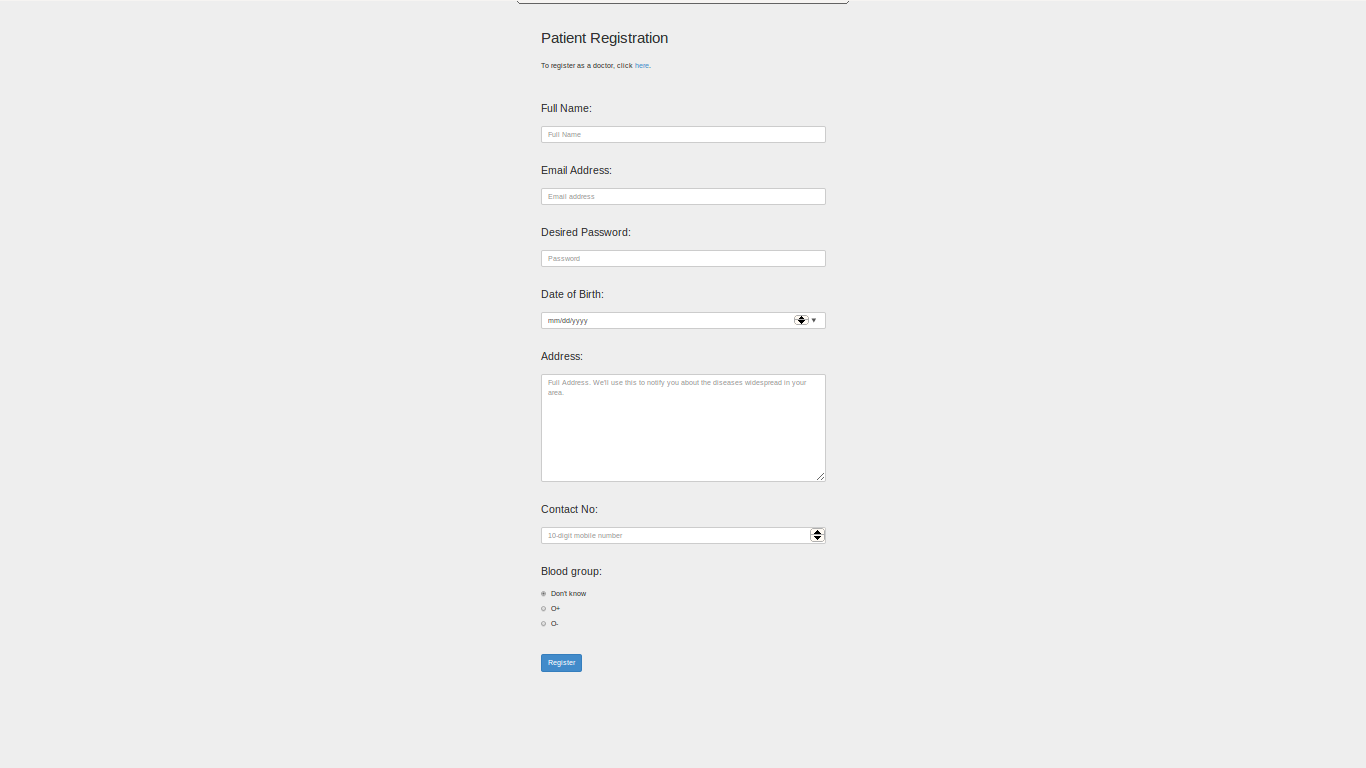
\includegraphics[width=0.95\columnwidth]{patient_reg.png}
	\caption{Patient Registration}
	\label{PR}
\end{figure}

For Patient registration refer Figure \ref{PR}.

\begin{figure}[!htbp]
	\centering
	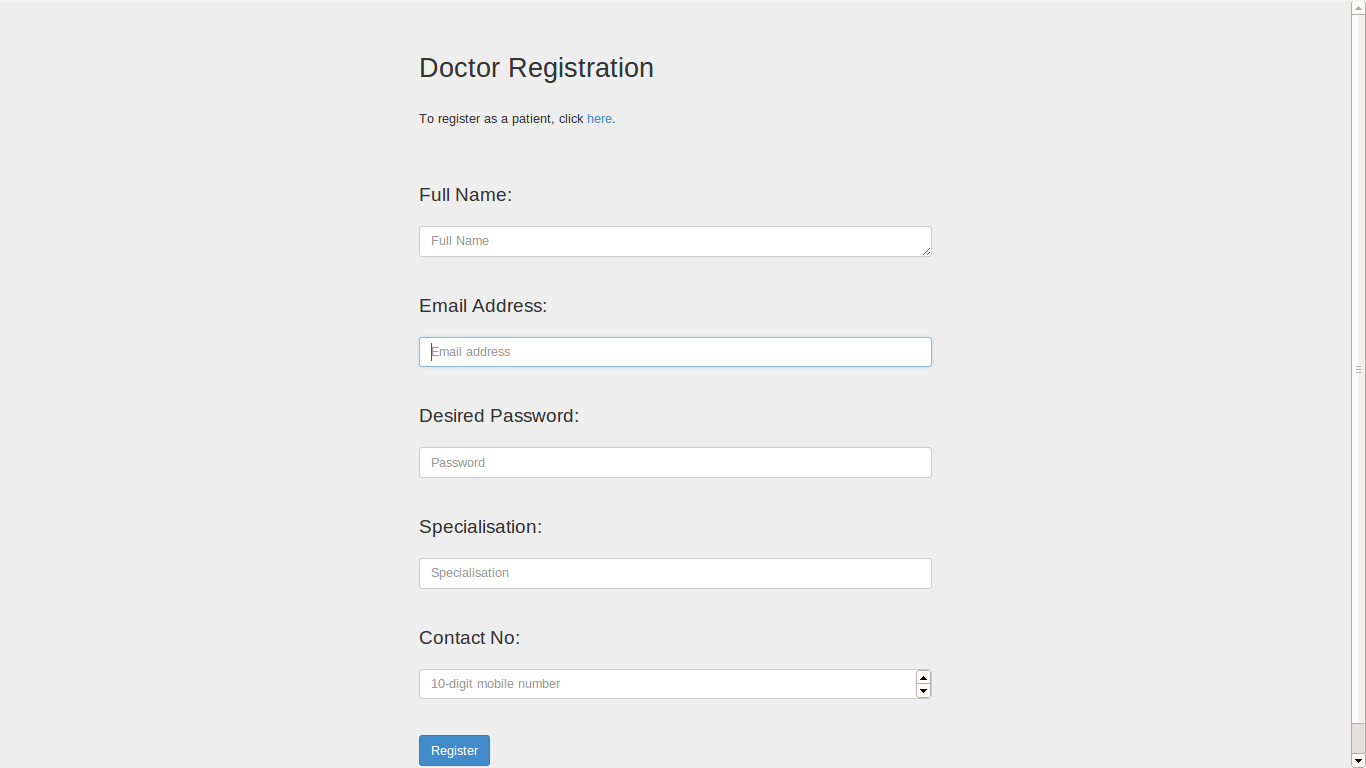
\includegraphics[width=0.95\columnwidth]{doctor_reg.png}
	\caption{Doctor Registraion}
	\label{DR}
\end{figure}

For doctor Registration refer Figure \ref{DR}.
\newpage
And we can have data like:\\
1) How many people were having any particular disease at a particular time?\\
\textit{select * from patientRecord2013 where disease = "diseasename" and date between '2013-01-01' and '2013-05-06';}\\
2) How many people are having disease on a particular day?\\
\textit{select * from patientRecord2013 where date between '2013-01-01' and '2013-05-06';}\\
3) What kind of symptoms are being discovered for a particular disease?\\
4) How is the trend of a disease change with respect to time?\\
5) What is the most popular disease at a time range for each year?\\
6) How the records of a doctor are changing with respect to the years?\\
7) Historic trends of the diseases of a patient. \\

\section{Conclusions}

We can use it as an online prescription form.It can be used to predict diseases from the given symptoms using machine learning techniques and we can also try to subscribe medicines to patients who cant buy costly medicines by looking at the constituents of the prescribed medicines.Significantly fewer errors found within personal health records.Faster care and decision making responses from assigned medical professionals.


\section*{References}

Directly type in bib entries.

Better is to use bibtex.

\end{document}